\section*{Техническое задание}
\addcontentsline{toc}{section}{Техническое задание}
Насос простого действия(рис. \ref{pic_pump}) состоит из кривошипно--ползунного механизма 1, 2, 3, ползун 3 которого является плунжером насоса, совершающим возвратно--поступательное движение в горизонтальном цилиндре 4 с автоматически действующими клапанами 5, 6.

Рабочий цикл такой установки совершается за один оборот кривошипа 1. При движении плунжера 3 вправо происходит всасывание жидкости в цилиндр при давлении ниже атмосферного $p_{min}$ и при движении поршня влево --- нагнетание жидкости в трубопровод при давлении $p_{max}$(см. индикаторную диаграмму рис. \ref{pic_ind_diagram}).

Коленчатый вал 1 кривошипно--ползунного механизма приводится во вращательное движение от электродвигателя 7 через планетарный редуктор с колёсами 8, 9, 10, 11, водило 12 и муфта 13. Для обеспечения требуемой неравномерности движения коленчатого вала имеется маховик 14.

Смазка подвижных соединений механизма установки осуществляется под давлением от масляного насоса 17 кулачкового типа(рис. \ref{pic_oil_pump}). Закон движения толкателя в пределах рабочего угла поворота кулачка $\varphi_{раб.}$ представлен на рис. \ref{pic_mov_push}. Вращение кулачка 17 осуществляется от кривошипа 1 через корригированные зубчатые колёса 15 и 16 с неподвижными осями вращения.

\begin{figure}[h!]
	\centering
	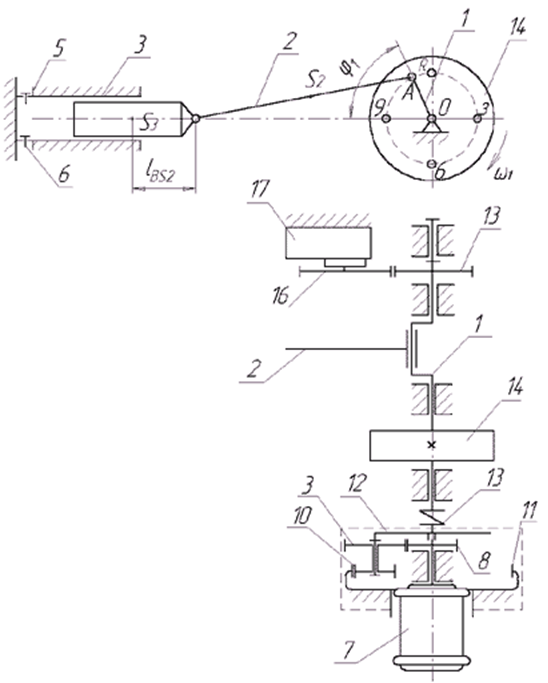
\includegraphics[width=0.5\linewidth]{pic/Source_mech}
	\caption{}
	\label{pic_pump}
\end{figure}

\begin{figure}[h!]
	\centering
	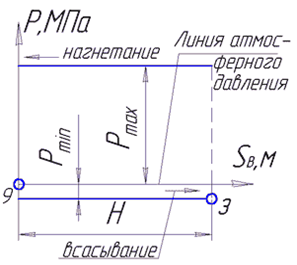
\includegraphics[width=0.3\linewidth]{pic/pressure}
	\caption{}
	\label{pic_ind_diagram}
\end{figure}

\begin{figure}[h!]
	\centering
	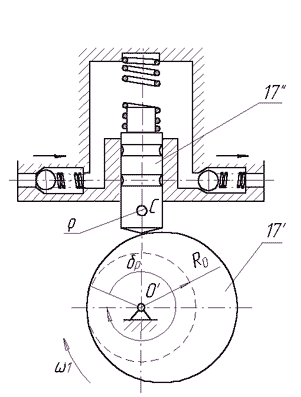
\includegraphics[width=0.4\linewidth]{pic/pump}
	\caption{}
	\label{pic_oil_pump}
\end{figure}

\begin{figure}
	\centering
	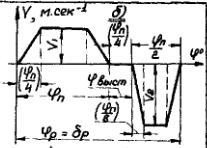
\includegraphics{pic/v(varphi)}
	\caption{}
	\label{pic_mov_push}
\end{figure}
